


%#######################################
\chapter{\label{sec:erh}Datengewinnung: Verkehrserhebungen}
%#######################################

Die Erhebung der Daten zum jeweiligen Sachverhalt ist ein wesentlicher
Bestandteil der Vorgehensweise in der \"Okonometrie. Insbesondere muss die Art
der Erhebung und die erhobenen Daten zum vorgesehenen
\"okonometrischen Modell 
passen. In diesem Kapitel werden neben der Erhebungsmethodik 
(Abschnitt \ref{sec:erh-meth}) die f\"ur die Verkehrs\"okonometrie
wichtigen  Datenkategorien
kurz vorgestellt: Verkehrsflussdaten (Abschnitt
\ref{sec:erh-fluss}), Daten zum Mobilit\"atsverhalten
(Abschnitt \ref{sec:erh-mobil}) und die direkte Nutzermessung
(Abschnitt \ref{sec:erh-nutzermessung}). Schlie\3lich wird in
Kap.~\ref{sec:conjoint} die wahlbasierte Conjoint-Analyse als
wichtigste Methode der direkte Nutzermessung im Verkehrskontext vorgestellt. 
Das Flussdiagramm \ref{fig:flussdiag-erhebung} zeigt als \"Ubersicht
die Einbindung der 
Datenerhebung in den allgemeinen Ablauf einer \"okonometrischen
Untersuchung.

%#############################
\begin{figure}
\fig{0.6\textwidth}{figsErh/flussdiag-komplett.eps}
\caption{\label{fig:flussdiag-erhebung}Eingliederung der Datenerhebung
in den allgemeinen Ablauf einer \"okonometrischen
Untersuchung.
}
\end{figure}
%#############################


%#######################################
\section{\label{sec:erh-ablauf}Ablauf einer Erhebung}
%#######################################

Eine Datenerhebung (vgl. Abb. \ref{fig:erh-flussdiag}) beginnt
 mit der Definition der statistischen
Einheiten (Merkmalstr\"ager), der r\"aumlich, zeitlich und sachlich
abzugrenzenden Grund\-gesamtheit und der nicht notwendigerweise
identischen Ziehungsgrundlage (Abschnitt \ref{sec:erh-meth}). 

Die zu
erhebenden Merkmale sind durch den Sachverhalt bzw. die
Modellspezifikation
 vorgegeben
und m\"ussen sowohl die exogenen als auch die endogenen Variablen
dieser Modelle enthalten. 

 %#############################
\begin{figure}
\fig{0.8\textwidth}{figsErh/flussdiag-ablauf.eps}
\caption{\label{fig:erh-flussdiag}Ablaufdiagramm einer
verkehrs\"okonometrischen Datenerhebung.
}
\end{figure}
%#############################



Anschlie\3end wird die Erhebung selbst spezifiziert: Meist wird man
als Ziehungsmthode eine Stichprobe w\"ahlen, deren Umfang man in
Abh\"angigkeit der angestrebten Ge\-nau\-ig\-keit festlegt
(vgl.  Statistik-Vorlesungen).
Die Modalit\"at der Stichprobe (Zufallsstichprobe,
geschichtete Stichprobe, Klumpenstichprobe)
richtet sich einerseits nach den zur Ver\-f\"u\-gung stehenden Mitteln
(Klumpenstichproben sind bei gleichem Umfang weniger aufw\"andig zu
erheben) und nach der Priorit\"at, welcher auf Repr\"asentativit\"at
und die Vermeidung
systematischer Verzerrungen gelegt wird (dann ist die
Zufallsstichprobe mit Entzerrung optimal).

Je nach Umfang und Komplexit\"at der Erhebung, 
der angestrebten R\"ucklaufquote und der verf\"ugbaren Mittel
w\"ahlt man die Erhebungsform aus (vgl, Abb. \ref{fig:erh-flussdiag}).  
Eine Erhebung in Form eines
pers\"onlichen Interviews ergibt die h\"ochste R\"ucklaufquote und die
h\"ochste Datenqualit\"at, da Missverst\"andnisse sofort gekl\"art
werden k\"onnen.

Nach Festlegung aller Erhebungsdetails wird zun\"achst an wenigen 
Probanden in einem \bfdef{Pre-Test} gepr\"uft, ob die Erhebung so
funktioniert wie vorgesehen, insbesondere, ob es Schwierigkeiten bei
der Fragenbeantwortung gibt und sich die Verweigererquote in den
anvisierten Grenzen
h\"alt. Nach Optimierung des Erhebungsprotokolls wird dann die
eigentliche Erhebung durch\-gef\"uhrt. 

Die Auswertung der Erhebung
beinhaltet schlie\3lich das Aufstellen der Systemgleichungen anhand des
vorgesehenen \"okonometrischen Modells. Diese Systemgleichungen dienen
dann als Ausgangspunkt f\"ur die Pamametersch\"atzung und den Test der
gewonnenen Aussagen.

%#######################################
\section{\label{sec:erh-meth}Erhebungsdesign}
%#######################################
Je nach Art der erhofften Aussagen bzw. der zu pr\"ufenden Hypothesen
wird die Erhebungsmethodik bez\"uglich folgender Kategorien
festgelegt:

%#############################
\begin{figure}
\fig{0.55\textwidth}{figsErh/Zeitdimension.eps}
\caption{\label{fig:Zeitdimension}Verschiedene Datenarten bzw. 
Erhebungsdesigns, aufgegliedert
bez\"uglich der Dimensionen Zeit, Stichprobenumfang (Achse
``Merkmalstr\"ager'') und Zahl der Merkmale bzw. typischer Umfang 
des Fragebogens (Achse ``Merkmale''). 
}
\end{figure}
%#############################

\subsection{Aggregierungsebene} 
Diese reicht von einer globalen
Untersuchung der relevanten Merkmale (\bfdef{makroskopische Ebene})
bis hin zur Ber\"ucksichtigung einzelner Merkmalstr\"ager
bzw. Individuen (\bfdef{mikroskopische Ebene}).  Den Spezialfall einer
Disaggregierung makroskopischer Daten nach Altersgruppen bezeichnet
man auch als \bfdef{Kohortendesign}. 

\subsection{Abgrenzung bzw. Zeit- und Merkmalstr\"agerdimension} 

Die Unterscheidungen werden in Abb. \ref{fig:Zeitdimension} veranschaulicht:
\bi
\item
\bfdef{Querschnittsdaten} werden zu einem festen Zeitpunkt oder
Zeitintervall erhoben und stellen quasi einen ``Schnappschuss'' der
Situation dar.\footnote{Dies hat nichts mit den ``Querschnittsdaten''
  der Verkehrsflussmessung durch station\"are Detektoren zu tun,
  vgl. Abschnitt~\ref{sec:erh-fluss}.} 
\item
Bei \bfdef{L\"angsschnittdaten} hingegen wird auch die Ver\"anderung
in der Zeit ber\"ucksich\-tigt. Dies kann in Form mehrerer
Querschnitterhebungen (\bfdef{Trend-Design}) erfolgen, welche in Zeitabst\"anden
von i.d.R. mehreren Jahren mit jeweils neuen Stichproben wiederholt werden. 
 Diese Methodik wird z.B.  bei den gro\3en
Mobilit\"atserhebungen SrV (System relevanter Verkehrserhebungen) und
MiD (Mobilit\"at in Deutschland) angewandt. Untersucht man hingegen
ein und dieselbe Stichprobe bzw. Personengruppe fortlaufend \"uber mehrere Jahre, spricht
man von \bfdef{Paneldaten}.\footnote{Die daran beteiligten Personen bezeichnet
man auch als Panel.} Um einen \"uberm\"a\3igen Ausfall der 
 im Panel enthaltenen Personen im Laufe der Zeit bzw. Fluktuationen zu
vermeiden, muss man bei solchen Befragungen jedoch die Zahl der erhobenen
Merkmale beschr\"anken, was in Abb. \ref{fig:Zeitdimension} durch eine
gegen\"uber der Querschnittserhebung reduzierten ``H\"ohe''
symbolisiert ist. Ferner ist bei einem Panel-Design der Umfang 
 der Stichprobe (in Abb. \ref{fig:Zeitdimension} symbolisiert
durch die ``Tiefe'' des entsprechenden Quaders) in der Regel geringer
als bei Querschnitts-Befragungen.

\item Zeichnet man hingegen nur einzelne Merkmale
kontinuierlich \"uber die Zeit auf, spricht man von einer \bfdef{Zeitreihe}.
\ei

\subsection{Ausma\3 der Kontrolle \"uber den Untersuchungsgegenstand}

\bi
\item \bfdef{Objektive Messung}. Die Daten werden hier
ohne jede Beeinflussung der zu untersuchenden Subjekte und Objekte
erhoben.\footnote{F\"ur Physiker: Abgesehen vom quantenmechanische
Messproblem.} 
Dies f\"uhrt zu maximaler Objektivit\"at, da durch
\"Uberpr\"ufung der Messger\"ate der
Wahrheitsgehalt der Messung im Prinzip immer getestet werden kann. 
Beispiele hierf\"ur sind Verkehrsz\"ahlungen
sowie Messung anderer objektiver Verkehrseigenschaften wie
Geschwindigkeit, Ver\-kehrsdichte etc.
(Abschnitt
\ref{sec:erh-fluss}). 

\item \bfdef{Erhebung tats\"achlicher Ereignisse durch
Befragung} (\emph{Revealed Choice}). Hier werden tat\-s\"ach\-lich realisierte Wahlentscheidungen wie
Wegekettenwahl, Verkehrs\-mittel\-wahl und Routenwahl und die relevanten
erkl\"arenden Variablen wie Alter, Ge\-schlecht, Zeit- und
Geldaufw\"ande f\"ur die verschiedenen Verkehrsmittel durch Befragung,
in der Regel au\3erhalb des Verkehrsraums, erhoben (Abschnitt
\ref{sec:erh-mobil}).  

Man erh\"alt eine
Vielzahl von Informationen, welche man durch eine objektive Messung
nie gewinnen kann: Man sieht einem vorbeifahrenden Kfz oder einem
Buspassagier  ja nicht an, wo der Ausgangspunkt und das Ziel des Weges
ist und welchem Zweck er dient. Andererseits ist der Wahrheitsgehalt
viel schwerer zu \"uberpr\"ufen. Fehler ergeben sich nicht nur durch
absichtliche Falschaussagen, sondern auch dadurch, dass sich die
befragten Personen  an
viele Details nicht oder nur unvollst\"andig erinnern.

\item \bfdef{Experientelles Design: Direkte Nutzermessung}
(\emph{Stated Choice}). Hier wird
nicht nach realisierten Entscheidungen gefragt, sondern
Gedankenexperimente durch\-gef\"uhrt nach dem Motto ``Wie w\"urden Sie
sich entscheiden, wenn Sie ein Kfz zur Verf\"ugung h\"atten und einen
Weg zur\"ucklegen m\"ussten, der zu Fu\3 30 min, mit dem Rad 10 min,
mit \"OPNV 20 min
und mit dem Kfz 8 min betr\"agt?  Im Gegensatz zur Erhebung
realisierter Entscheidungen hat hier der Experimentator viele der
exogenen Variablen unter Kontrolle und kann sie genau in den
interessanten Bereich bringen. Hingegen sinkt naturgem\"a\3 die
Objektivit\"at. Verzerrungen und systematische Fehler lassen sich kaum
kontrollieren. N\"aheres in den Abschnitten ab
\ref{sec:erh-nutzermessung}).

\item \bfdef{Kombiniertes Design}
Hier werden Revealed-Choice Daten als Angelpunkt oder
\bfdef{Pivot} einer Stated-Choice Befragung derselben Personen
genommen, um den Stated-Choice Fragebogen zu
optimieren. Typischerweise wird als Referenz der durch die Revealed
Choice Befragung aufgedeckte wahre Sachverhalt verwendet und dieser
dann schrittweise ver\"andert.
\ei

\subsection{Ziehungsmethode} 

Bei jeder \"okonometrischen
Untersuchung muss man zun\"achst die Merkmalstr\"ager und deren 
\bfdef{statistische Gesamtheit}
bzw.\bfdef{Grund\-gesamtheit} 
definieren. Dies geschieht (vgl. Statistik-Grundvorlesung) durch 
\bi
\item \bfdef{r\"aumliche Eingrenzung} (z.B. Untersuchungsgebiet
Deutschland oder Dresden),
\item \bfdef{zeitliche Eingrenzung} (Zeitpunkt oder Zeitraum,
z.B. Sommer 2008)
\item \bfdef{sachliche Eingrenzung} (z.B. nur erwachsene Personen,
einschlie\3lich Ausl\"ander, die in Deutschland leben aber
ausschlie\3lich Deutsche, die im Ausland leben).
\ei
Die Ziehungsmethode wird dann charakterisiert durch 
\bi
\item Die \bfdef{Ziehungsgrundlage}. Diese ist bei objektiven Messungen eine
Teilmenge der r\"aumlichen und zeitlichen Abgrenzung (z.B. die mit
Detektoren ausgestattete Streckenabschnitte) und bei Befragungen meist ein Register, z.B. das
Einwohnermelderegister oder das Kfz-Zulassungsregister. Die
Ziehungsgrundlage muss nicht identisch zur
Grund\-gesamtheit sein. Vielmehr kann es sich um eine Obermenge handeln
(z.B. Einwohnerregister bei einer aus Motorradfahrern bestehenden
Grund\-gesamtheit), um einer Untermenge (viele Gewohnheiten 
deutscher Einwohner werden anhand einer repr\"asentativen
Durchschnittsstadt erhoben), oder um eine ab\-ge\-lei\-te\-te Menge
(z.B. Einwohnerregister bei einer aus Haushalten bestehenden
Grund\-gesamtheit).\footnote{Dieser Sachverhalt wurde in der Bachelor-Vorlesung
in Verkehrs\"okonometrie 
ausf\"uhrlich behandelt.}
\item 
\bfdef{Vollerhebung} oder \bfdef{Stichprobe}. Vollerhebungen sind extrem aufw\"andig
und kommen (abgesehen von der Volksz\"ahlung) nur f\"ur kleine
statistische Gesamtheiten in Frage. Bei der Stichprobe wiederum
unterscheidet man im Wesentlichen die \bfdef{Zufallsauswahl}, die
\bfdef{Proportionalauswahl} (geschichtete Stichprobe)  und die \bfdef{Klumpenauswahl}
\ei

\subsection{Modalit\"at der Erhebung}

Bei Messungen objektiver Merkmale
wird die Erhebung in der Regel automatisch durch\-gef\"uhrt, sie kann
aber auch h\"andisch z.B. durch Z\"ahlger\"ate, Notebookeingabe oder Strichlisten
erfolgen. Wichtige Erhebungsmodi bei der Befragung sind 
\bi
\item Pers\"onliche Befragung durch eine Betreuungsperson,
\item schriftlich,
\item telefonisch,
\item und per Internet.
\ei
Kombinationen (z.B. telefonisches Nachfragen bei Ausbleiben einer
schriftlichen Antwort und Hotlines) sind ebenfalls \"ublich.



%#############################
\begin{figure}
\fig{1.04\textwidth}{figsErh/ganglinien-A9munich.eps}
\caption{\label{fig:ganglinien}Verkehrsbelastungs- und
Geschwindigkeitsganglinien auf der A9-S\"ud bei M\"unchen. Der
Ausschnitt zeigt, dass in der morgendlichen Rush-Hour
Stop-and-Go-Verkehr herrscht.
}
\end{figure}
%#############################

%#######################################
\section{\label{sec:erh-fluss}Beispiel einer objektiven Messung: Verkehrsflussdaten}
%#######################################

Verkehrsflussdaten werden direkt im Verkehrsgeschehen an festen
Orten erhoben. In der Regel sind sich die Verkehrsteilnehmer
(Fu\3g\"anger, Radfahrer, Autofahrer) der Erhebung
nicht bewusst.

\subsection{Mesung}
 Die Erfassung erfolgt in der Regel auf einer der
folgenden Arten:
\bi
\item Personen mit Z\"ahlger\"aten oder Strichlisten (Stadtverkehr,
Untersuchungen f\"ur spezielle Zwecke),
\item Videoaufzeichnung mit anschlie\3ender manueller  Auswertung,
\item automatisch Messung an 
\bfdef{Messquerschnitten}\footnote{Manchmal werden auf diese Weise
erhobene  Verkehrsflussdaten
als ``Querschnittsdaten'' bezeichnet, da sie sich auf den Querschnitt
einer Stra\3e beziehen. In Abschnitt \ref{sec:erh-meth}
wurde dieser Begriff jedoch  definiert als Daten, welche
 zu einem Zeitpunkt bzw. einem
Zeitraum erhoben wurden, w\"ahrend die hier gemeinten Daten der
Kategorie ``Zeitreihe'' zuzuordnen sind.
Um Verwechslungen zu vermeiden, wird 
im Folgenden der Begriff ``Querschnittsdaten'' nur in der in 
 Abschnitt \ref{sec:erh-meth} eingef\"uhrten
Bedeutung als ``Schnappschuss zu einem Zeitpunkt bzw. Zeitraum'' verwendet.}
Die Messung kann dabei erfolgen durch
\bi
\item \bfdef{pneumatische Z\"ahler}: 
Vor allem Stadtverkehr als  tempor\"are Anwendung,
\item  \bfdef{Induktionsschleifen} oder Infrarot-Messung: 
In der Regel permanente Anwendung, im Stadtverkehr
z.B. als Sensor f\"ur verkehrsabh\"angig gesteuerte
Lichtsignalanlagen, auf der Autobahn zur Verkehrslagesch\"atzung und
als Sensor f\"ur Verkehrsbeeinflussungsanlagen
\item Videocamera mit automatischer Auswertung (Tracking). Damit
k\"onnen neben Kfz-Str\"ome auch z.B. Fu\3g\"angerstr\"ome erfasst werden.
\ei
\ei
\noindent
Typische  erhobenen Merkmale sind die Folgenden:
\bi
\item  Verkehrsfluss im engeren Sinne, d.h. Zahl der Fu\3g\"anger oder
Kfz, welche einen bestimmten Querschnitt pro Zeitintervall
\"uberqueren,
\item Geschwindigkeit, entweder \"uber Zeitintervalle aggregiert
 oder als Einzelmerkmal (nur bei Doppelinduktionsschleifen oder aus
Videodaten),
\item evtl. Art der Fahrzeuge oder zumindest die Fahrzeugl\"ange
\item evtl. Trajektorien in der N\"ahe des Querschnitts.
\ei

\noindent
Abbildung \ref{fig:ganglinien} Zeigt als Beispiel den Verkehrsfluss
und die in Minutenintervallen aggregierte Geschwindigkeit von
Messquerschnitten auf der Autobahn A9-S\"ud n\"ordlich von M\"unchen. Man
sieht insbesondere, das es in der morgendlichen Rush-Hour (Maximum im
Fluss) zu einem Stau (Zusammenbruch der Geschwindigkeit) kommt. In der
Detailansicht der Geschwindigkeits-Zeitreihe (rechts) sieht man, dass
es sich um
die Stauart ``Stop-and-Go-Verkehr'' handelt.

%#############################
\begin{figure}
\fig{0.75\textwidth}{figsErh/bemessungsverkehrsstaerke.eps}
\caption{\label{fig:bemessungsverkehrsstaerke}Zur Definition der
Bemessungsverkehrsst\"arke $Q\sub{bem}$
}
\end{figure}
%#############################

\subsection{Tagesganglinien und Bemessungsverkehrsst\"arke}

Die \"uber einen Tag aufgenommene Zeitreihe des Flusses bezeichnet man
auch als \bfdef{Tagesganglinie}. Nat\"urlich h\"angt
die Tagesganglinie auch vom Wochentag und (in geringerem Umfang) 
von der Saison (Sommer, Winter etc) sowie von Sondersituationen
(z.B. Ferienanfang, Fu\3ballspiel) ab. Man definiert deshalb
verschiedene F\"alle, z.B. ``Normalwerktag''=Dienstag bis Donnerstag,
Freitag, Samstag usw., jeweils in ``normalen'' Wochen und Wochen mit
Sondersituationen. 

In ihrer Gesamtheit geben die Tagesganglinien 
 Aufschluss \"uber die St\"arke und
zeitliche Verteilung der Verkehrsbelastung. Insbesondere l\"asst sich
damit die sogenannte \bfdef{Bemessungsverkehrsst\"arke} als Quantil
der Verkehrsnachfrageverteilung definieren
(vgl. Abb. \ref{fig:bemessungsverkehrsstaerke}): 

\maintext{Die  \bfdef{Bemessungsverst\"arke} einer Richtungsfahrbahn 
ist die Verkehrsnachfrage
(in Kfz/h oder Kfz/h/Fahrstreifen), welcher im statistischen Mittel
nur an 30 Stunden im Jahr \"uberschritten wird.
}

Hintergrund ist, dass man aus
\"okonomischen Gr\"unden die Kapazit\"at der Stra\3en nicht nach der
maximal zu erwarteten Nachfrage dimensioniert, sondern man vielmehr
einen  gewissen Zeitanteil mit
Strecken\"uberlastung und daraus resultierenden Staus ``in Kauf''
nimmt.\footnote{Dasselbe Prinzip gilt bei der Bemessung von
Hochwasserverbauungen: Die Schutzma\3nahmen schlie\3en regelm\"a\3ig
Ereignisse vom Typ ``HW200'' oder ``HW1000'' aus, also Hochwasser, welche im Mittel
nur alle 200 bzw. 1\,000 Jahre vorkommen.}

\verstaendnisbox{Welchem Quantil der Flussverteilung entspricht obige
Definition der Bemessungsverkehrsst\"arke?
}





%#############################
\begin{figure}[h!]
\fig{0.45\textwidth}{figsErh/SrV-Stichprobe.eps}
\caption{\label{fig:SrV-Stichprobe}Visualisierung der 
Grund\-gesamtheit (hellblau) und der Stichprobe (dunkelrot)
bei der Mobilit\"atserhebung SrV. Grund\-gesamtheit und
Stichprobe sind dabei als zweidimensionale Mengen in den Dimensionen
``statistischen Einheiten'' (Haushalte 1 bis $N$ mit $N$ der Zahl der
Haushalte in der Grund\-gesamtheit) und der Zeit aufgetragen.
}
\end{figure}
%#############################

%#############################
\begin{figure}
\fig{0.92\textwidth}{figsSrV/SrV2003_Haushaltsfragebogen.eps}
\caption{\label{fig:SrV-Haushalt}Haushaltsfragebogen der
Mobilit\"atserhebung SrV 2003.
}
\end{figure}
%#############################

%#######################################
\section{\label{sec:erh-mobil}Beispiel zu einer Revealed-Choice
  Erhebung: SrV}
%#######################################
Mobilit\"atsdaten beinhalten alle exogenen und endogenen Variablen des
jeweils verwendeten \"okonometrischen Modells, also im Gegensatz zu den
Verkehrsflussdaten nicht nur das Ergebnis in Form von
Verkehrsbewegungen, sondern auch das Wozu, das Woher-Wohin, sowie die
das Subjekt (den Verkehrsteilnehmer) und seinen/ihren Hintergrund n\"aher beschreibenden
sozio\"okonomischen Variablen. Damit ist klar, dass eine Erhebung
nicht automatisch, sondern nur
durch \textit{Befragung} durch\-gef\"uhrt werden kann. 


Die Erhebung von
Mobilit\"atsdaten soll am Beispiel der in Zusammenarbeit mit der TU
Dresden (Prof. Ahrens) durch\-gef\"uhrten Erhebung \bfdef{System relevanter
Verkehrsbefragungen} (SrV) verdeutlicht werden.
Die \bfblack{statistische Gesamtheit}
wird charakterisiert durch


%#############################
\begin{figure}
\fig{0.92\textwidth}{figsSrV/SrV2003_Personenfragebogen.eps}
\caption{\label{fig:SrV-Personen}Personenfragebogen der
Mobilit\"atserhebung SrV 2003.
}
\end{figure}
%#############################

\bi
\item Statistische Einheit: (i) Haushalte
(Abb. \ref{fig:SrV-Haushalt}), (ii) Personen
(Abb. \ref{fig:SrV-Personen}) 
\item R\"aumliche Abgrenzung: 34 Ausgew\"ahlte St\"adte und Gemeinden in Deutschland,
u.a. Dresden
\item Zeitliche Abgrenzung: Alle ``mittleren Werktage''
(Dienstag-Donnerstag) im Jahr 2003
\item Sachliche Abgrenzung: Alle in den jeweiligen St\"adten wohnende
Personen, also einschlie\3lich Kinder und Ausl\"ander.
\ei
%
Die \bfblack{Stichprobe} wird aus den \textit{Einwohnermelderegistern}
durch Auswahl von \textit{Haushalten}  per \textit{Zufallsauswahl}
gezogen.  Aus den gew\"ahlten Haushalten werden \textit{alle Peronen}
einbezogen.
Der \textit{Stichprobenumfang} betr\"agt etwa 6000 Personen (etwa
3000) Haushalte im Gro\3raum Dresden und etwa ein Sechstel davon in
den meisten \"ubrigen St\"adten/Gemeinden.

Die Stichprobe ist aber nicht nur in der Dimension der statistischen
Einheiten ein Teil der Grund\-gesamtheit, sondern auch in der zeitlichen
Dimension: Erhebungen wurden nur im April und Mai 2003 durch\-gef\"uhrt
und es wurden pro Haushalt bzw. Person  nur die Mobilit\"atsdaten f\"ur
einen einzigen \textit{Bezugstag} erhoben (vgl. Abb. \ref{fig:SrV-Stichprobe})


%#############################
\begin{figure}
\fig{0.95\textwidth}{figsSrV/SrV2003_Wegefragebogen_p1.eps}
\caption{\label{fig:SrV-Wege}Wegefragebogen der
Mobilit\"atserhebung SrV 2003.
}
\end{figure}
%#############################

Das \bfblack{Erhebungsdesign} sieht eine Erhebung
\textit{tats\"achlicher Ereignisse} auf \textit{individueller}
Ebene im \textit{Trend-Design} vor, d.h. eine Querschnittserhebung in
gewissen (mehrj\"ahrigen) Zeitabst\"anden (ab 1972; die letzten beiden
Erhebungen in den Jahren 2003 und 2008).
Die \bfdef{Modalit\"at der Erhebung} ist entweder ein
\textit{Telefoninterview} oder eine \textit{schriftliche Befragung per
Fragebogen}.

Die erhobenen \bfblack{Merkmale} der Personen k\"onnen nach mehreren Kategorien
unterschieden werden:
\bi
\item \bfdef{Allgemeine soziodemografische und sozio\"okonomische
Merkmale}: Wohnort und -Lage, Zugeh\"origkeit zu Haushalt mit  $n$ Personen, 
Alter, Ge\-schlecht, Beruf, Ausbildungsniveau usw. Diese Merkmale werden
im Haushalts- und Personenfragebogen erhoben
(Abb. \ref{fig:SrV-Haushalt} bzw. \ref{fig:SrV-Personen}).
\item \bfdef{Mobilit\"atsbezogene sozio\"okonomische Merkmale}:
F\"uhrescheinbesitz, Kfz- und Fahradverf\"ugbarkeit, Besitz von
\"OPNV-Dauerkarten, Entfernung zur n\"achsten \"OPNV-Haltestelle. 
Diese Merkmale werden
ebenfalls im Haushalts- und Personenfragebogen erhoben.
\item \bfdef{Aktivit\"atenbezogene Merkmale}: Zahl der Wege
(definiert als zielgerichtete Ortsver\"anderung im \"offentlichen
Verkehrsraum) sowie der
Wegezweck (die Zielaktivit\"at). Merkmale dieser und der folgende
Datenkategorie werden in den Wegefrageb\"ogen (Abb. \ref{fig:SrV-Wege})
erhoben.
\item \bfdef{Wege- bzw. alternativenbezogene Merkmale}: Start und
Zielpunkt eines Weges; Gew\"ahltes
Verkehrsmittel sowie Reisezeit, Reiseweite und die Kosten des gew\"ahlten
Verkehrsmittels f\"ur diesen Weg. Aus diesen und den sozio\"okonomischen
Merkmalen sowie den Merkmalen der Infrastruktur  
lassen sich auch Sch\"atzungen f\"ur Reisezeit, Reiseweite und
die Kosten der verf\"ugbaren Verkehrsmittelalternativen ableiten.
\ei
Je nach Modell handelt es sich dabei um exogene oder endogene
Variable. F\"ur ein Verkehrsmittelwahlmodell ist beispielsweise nur das gew\"ahlte
Verkehrmittel eine endogene Variable, w\"ahrend alle anderen Merkmale
die Rolle von exogenen Variablen spielen.
Bei Modellen  der Verkehrserzeugung  sind die beiden ersten
Kategorien exogen, die  aktivit\"atenbezogenen Merkmale  endogen und
die Wege- bzw. alternativenbezogene Merkmale nicht relevant.

F\"ur die Modellierung ist es relevant, dass die Merkmale verschiedene Skalierungen aufweisen,
z.B. dichotom bzw. zweiwertig wie das Ge\-schlecht, allgemein
nominalskaliert (z.B. Beruf, gew\"ahltes Verkehrsmittel),
ordinalskaliert (z.B. Ausbildungsgrad,
Kfz-Ver\-f\"ug\-bar\-keit) oder kardinalskaliert (z.B. Alter, Reisezeiten und
-weiten). Ferner ist f\"ur die Modellierung wesentlich, dass einige
Variable personengebunden  sind und sich von Tag zu Tag nicht 
\"andern\footnote{Zumindest innerhalb des pers\"onlichen Planungszeithorizonts f\"ur die
allt\"aglichen Ziel -und Verkehrsmittelentscheidungen. Auf l\"angeren Zeitskalen
finden nat\"urlich durch Umz\"uge, Anschaffungen, berufliche Ver\"anderungen oder auch
schlicht durch  das \"Alterwerden Ver\"anderungen statt.}
(sozio\"okonomische Merkmale), andere sind personengebunden und
\"andern sich t\"aglich (aktivit\"atenbezogene Merkmale). Schlie\3lich
h\"angen die wege- und alternativenbezogenen Merkmale nicht nur von
der Person und dem Tag, sondern auch vom Weg und dem Verkehrmittel ab.



%#######################################
\section{\label{sec:erh-nutzermessung}Direkte Nutzermessung:
  Experimentelles Design}
%#######################################

In den im vorherigen Abschnitt besprochenen
Mobilit\"atserhebungen werden tats\"achlich realisierte Entscheidungen
abgefragt und daraus dann mit Hilfe von Modellen der diskreten Wahltheorie
Schlussfolgerungen \"uber die Bewertungen der verschiedenen
Alternativen gezogen. Deshalb nennt man diese Erhebungen auch
\bfdef{revealed preference}, also ``aufge\-deck\-te Pr\"aferenzen'' (bei
der Bewertung des Nutzens). Man kann aber die Pr\"aferenzen, also
die Gewichtung der Anteile der Nutzenfunktion, direkt messen, indem
man die befragten Personen mit \emph{hypothetischen Situationen}
konfrontiert, also \emph{Gedankenexperimente} durch\-gef\"uhrt. Es gibt
drei Varianten dieser auch als  \bfdef{experimentelles Design}
bekannten Versuchsanordnung: 
\bi
\item[(a)] \bfdef{Stated preference}. Verschiedene Alternativen oder
auch Aspekte bzw. Merkmale eines Angebots
werden mit einer Rangskala bewertet. Beispiel: \textit{Bewerten Sie allgemein
die Attraktivit\"at des \"OV-Angebots in Ihrer Stadt mit Schulnoten
von 1 bis 6.}
\bfblack{Likert-Skala 1-5 mit Bild einfuegen!}
% Welche Bewertung w\"urden Sie dem \"OV auf Ihrem
%Arbeitsweg geben? Wie wichtig sind ihnen Taktfolge, P\"unktlichkeit,
%Sauberkeit, Bequemlichkeit, Sicherheit und der Fahrpreis? Vergeben Sie
%auch hier jeweils Schulnoten.}

\item[(b)] \bfdef{Stated ranking}. Hier werden
Alternativen nach der  Rangfolge ihrer Attraktivit\"at (beste
Alternative, zweitbeste, etc) 
geordnet: \textit{Was ist Ihnen im \"offentliche Nahverkehr wichtig:
  Ordnen Sie die Kriterien Fahrpreis, Fahrzeit, Zuverl\"assigkeit und
  Sicherheit nach Ihrer pers\"onlichen Wichtigkeit.}

\item[(c)] \bfdef{Stated choice}. Hier wird nur nach der besten aus
zwei oder mehr Alternativen gefragt. F\"ur zwei Alternativen ist dies
\"aquivalent zum Stated Ranking. Beispiel: \textit{F\"ur den
  Tageseinkauf in einem \unit[3]{km} entfernten Supermarkt 
stehen Ihnen ein Kfz (Reisezeit \unit[10]{min}), das Rad
(\unit[15]{min}) sowie der Bus (\unit[15]{min} und Kosten 2 \euro{}) zur
Verf\"ugung. Welches Verkehrsmittel
w\"ahlen Sie?}

\ei

 Die \textit{Vorteile} dieser Erhebungsmethode sind
\bi
\item Einzelne Einflussfaktoren (Zeit, Geld, Flexibilit\"at) sind
leichter separierbar und ihre relative Gewichtung (z.B. Zeit/Geld
Faktor) direkt ermittelbar,
\item da man die Versuchanordnung und die exogenen Variablen unter
  Kontrolle hat, kann man genau das erfragen, was f\"ur die
  Untersuchung relevant ist.
\item man kann auch das Wahlverhalten nach Realisierung von geplanten
  Ma\3nahmen erfragen, f\"ur die es naturgem\"a\3 keine \emph{Revealed
  Choice} Erhebung geben kann. 
\ei

Es gibt aber auch \textit{Nachteile}:
\bi
\item Subjektive Bewertung einer oft hypothetischen Situation. Die
Probanden entscheiden sich bisweilen anders, als sie es bei einer
``echten'' Entscheidung tun w\"urden,
\item Leichter manipulierbar.
\ei




\section{\label{sec:conjoint}Konkretes Anwendungsbeispiel:
  Wahlbasierte Conjoint-Analyse} 

\subsection{Allgemeines}

Die \textit{Stated-Choice} Befragung liefert die empirische Grundlage der
wahlbasierten Conjoint-Analyse. Allgemein bezeichnet die
\bfdef{Conjoint-Analyse} (Akronym aus dem Englischen:
\emph{ \underline{con}sidered \underline{joint}ly)}, ganzheitlich betrachtet)
ein in der Psychologie entwickeltes und nun haupts\"achlich im
Produktmarketing angewandtes multivariates Verfahren zur gemeinsamen
Bewertung der St\"arke verschiedener Einflussfaktoren auf den Gesamtnutzen
eines bestimmten realen oder fiktiven Produkts.

F\"ur die Verkehrs\"okonometrie, insbesondere zur Analyse der Einflussfaktoren
verkehrsbezogener Wahlentscheidungen, ist eine Weiterentwicklung der traditionellen
Conjoint-Analyse, die \bfdef{wahlbasierte Conjoint-Analyse}, relevant. Dabei
werden den befragten Personen mehrere Alternativenmengen vorgelegt, woraus im
\emph{stated-choice} Verfahren jeweils die (hypothetisch) gew\"ahlte
Alternative abgefragt wird. In jeder Alternativenmenge (engl. \bfdef{\emph{choice
  set}}) werden alle oder einige Alternativen mit jeweils genau definierten und von
\emph{choice set} zu \emph{choice set} im allgemeinen unterschiedlichen
Attributwerten zur (hypothetischen) Wahl gestellt: 
\bi
\item Bei der Wahlentscheidung zum Autokauf k\"onnen die Attribute
  (Merkmale, Einflussfaktoren, exogene Variable)
  beispielsweise den Kaufpreis, die Marke, den Typ (Flie\3heck, Kombi, SUV,
  Van, Zweisitzer ...), den Verbrauch, die Motorleistung,
  den Wiederverkaufswert nach 5 Jahren, die Zuladungskapazit\"at und vieles
  mehr enthalten.
\item Bei der Verkehrsmittelwahl sind wichtige Einflussfaktoren sicherlich der
  Modus als solches, die
  (Grenz-)kosten, die Reisezeit und die Zuverl\"assigkeit.
\ei
Dieser Fragebogen wird dann mit den Mitteln der in
Kapitel~\ref{sec:choice} vorgestellten \bfdef{diskreten Wahltheorie}
analysiert.

\subsection{\label{sec:erh-studiBsp}Beispiel: Studentenbefragung}
Als einfaches Beispiel zur wahlbasierten Conjoint-Analyse  kann als
Input eine
\textit{Stated-Choice} Befragung zur Verkehrsmittelwahl 
unter 75 Studenten einer vergangenen Vorlesung dienen. Die Ergebnisse
sind in der Tabelle \ref{tab:statedChoice} widergegeben. Dabei wird
ein bestimmter Wegezweck angenommen, welcher von den Probanden gut
vorstellbar ist (hier: der Weg von zu Hause zur Uni).  Das Stated-Choice
Experiment besteht nun darin, unter den in der
Tabelle dargestellten hypothetischen Situationen (\emph{choice sets})
je eine Entscheidung 
zu treffen zwischen folgenden Alternativen:
\bi
\item Alternative 1: zu Fu\3 oder mit dem Rad, je nach pers\"onlicher Vorliebe,
\item Alternative 2: Mit dem \"OPNV.
\ei
In den verschiedenen Situationen sind die Alternativen
unterschiedlich gut ausgestattet, also mehr oder weniger attraktiv:
Als exogene (beeinflussende) Variablen wurden hier lediglich die
generischen Variablen
\bi
\item Komplexe (Haust\"ur-zu-Haust\"ur) Reisezeiten in Minuten
\item Zusatzkosten (Ad-Hoc Kosten) einer \"OV Fahrt in \euro{}
\ei
angenommen. Dabei kann die komplexe Reisezeit, obwohl eine generische
Variable, auch \emph{alternativenspezifisch} formuliert werden, indem
unterschiedliche Bewertungen f\"ur jeden Verkehrsmodus angenommen
werden (``eine Minute
im \"OV'' ist weniger unangenehm als eine zu Fu\3''). 
Mit Zusatzkosten sind die zus\"atzlichen Kosten gemeint, die
unabh\"angig von ggf. vorhandenen Dauerkarten auf jeden Fall bezahlt
werden m\"ussen. Die
Probanden m\"ussen sich dies als hypothetische Situation vorstellen, 
auch wenn in der Realit\"at das Semesterticket alles deckt.
Sozio\"okonomischen Variablen wurden hier nicht erhoben, aber einige
sozio\"okonomische Merkmale sind aufgrund der Zusammensetzung der
befragten Personen ohnehin bekannt, z.B. ``ist Student'' oder ``nicht
zu alt''.

%#############################################
\begin{table}
\begin{center}
\textbf{SS 2009}
\begin{tabular}{|c||c|c||r|r|r|r|r|}
\hline
\myBox{5em}{Hypoth.\\Situation} & 
\myBox{5em}{Altern. 1:\\Fu\3/Rad}  & 
\myBox{6em}{Altern. 2:\\ \"OPNV} & 
\myBox{2em}{Wahl\\$h_1$} & 
\myBox{2em}{Wahl\\$h_2$} &
\myBox{3em}{Logit:\\$(h_1)\sub{pred}$} &
\myBox{3em}{Logit:\\$(h_2)\sub{pred}$}\\ \hline\hline
1 & \unit[30]{min} & \unit[30]{min} + \unit[0]{\euro{}} & 5 & 70 & 3.9& 71.1\\ \hline
2 & \unit[30]{min} & \unit[40]{min} + \unit[0]{\euro{}} & 21 & 54 & 26.0& 49.0\\ \hline
3 & \unit[30]{min} & \unit[50]{min} + \unit[0]{\euro{}} & 63 & 12 & 62.7& 12.3\\ \hline
4 & \unit[30]{min} & \unit[60]{min} + \unit[0]{\euro{}} & 75 & 0 & 73.5& 1.5\\ \hline
5 & \unit[30]{min} & \unit[30]{min} + \unit[1]{\euro{}} & 26 & 49 & 19.8& 55.2\\ \hline
6 & \unit[30]{min} & \unit[30]{min} + \unit[2]{\euro{}} & 50 & 25 & 52.5& 22.5\\ \hline
7 & \unit[30]{min} & \unit[30]{min} + \unit[3]{\euro{}} & 70 & 5 & 70.4& 4.6\\ \hline
8 & \unit[20]{min} & \unit[30]{min} + \unit[0]{\euro{}} & 35 & 40 & 38.5& 36.5 \\ \hline
9 & \unit[15]{min} & \unit[30]{min} + \unit[0]{\euro{}} & 64 & 11 & 61.7& 13.3\\ \hline
\end{tabular}

\end{center}
\caption{\label{tab:statedChoice}Ergebnis des
Stated-Choice-Experiments in der
 \"Okonometrie-Vorlesung im SS 2009. Die letzten beiden Spalten geben die vom
kalibrierten Logit-Modell vorausgesagten Entscheidungszahlen an. Das
Logit-Modell und seine Parametersach\"atzung werden in
Kapitel~\ref{sec:choice} besprochen.
}
\end{table}
%#############################################

\noindent
Die Auswertung direkter Nutzermessungen wird mit der erst sp\"ater in
Kapitel \ref{sec:choice} besprochenen \bfdef{Diskreten Wahltheorie}
durch\-gef\"uhrt. Hier wird die Anwendung  dieser m\"achtigen
und f\"ur die Verkehrs\"okonometrie zentralen Theorie deshalb nur kurz
vorgestellt:
\bi
\item Zun\"achst wird f\"ur jede Alternative $k$ eine parameterlineare 
kardinalskalierte 
Nutzenfunktionen $U_k=V_k+\epsilon_k$ formuliert -- in Analogie zu den
Regressionsmodellen, nur dass der i.i.d. \bfdef{Zufallsnutzen} $\epsilon_k$
nun nicht nur einer Gau\3verteilung sondern auch anderen Verteilungen
gehorchen kann.
\item Die Alternative mit dem h\"ochsten
  Gesamtnutzen wird gew\"ahlt (\emph{Homo Oeconomicus}). Dies resultiert
  wegen des Zufallsnutzens in 
  \emph{Auswahlwahrscheinlichkeiten} $P_k$, welche als exogene
  Variable der diskreten Wahltheorie angesehen werden k\"onnen.
\ei
%
F\"ur die Erstellung der \bfdef{deterministischen} Nutzenfunktionen $V_k$ und die
Erhebung der geeigneten Merkmale gelten deshalb folgende Prinzipien:
\bi
\item \bfdef{Translationsinvarianz}: Man kann zu den
  Nutzenfunktionen aller Alternativen 
einen festen Wert hinzuaddieren, ohne dass sich das
  Ergebnis  \"andert.
\item \bfdef{Skaleninvarianz}: Wegen dem Prinzip \emph{the winner takes
  it all}, also einer Entscheidung auf Basis einer 
Ordinalskalierung (``besser oder schlechter''), \"andert sich das
Ergebnis nicht, wenn man die
Nutzenfunktionen einer beliebigen  streng
  monotonen Funktion unterwirft, solange dies f\"ur alle
  deterministischen \emph{und} stochastischen Nutzenanteile aller
  Alternativen geschieht. Insbesondere kann man die Nutzenfunktionen
  mit einer festen positiven Konstante multiplizieren, so dass der
  deterministische Nutzen \emph{in Einheiten der Standardabweichung
    des Zufallsnutzens} gemessen wird.
\ei

Mit den erhobenen exogenen Variablen $T_1$, $T_2$ (komplexe
Reisezeiten f\"ur Fu\3/Rad bzw. \"OV) und $K_2$ (\"OV Ad-Hoc-Kosten)
ergibt dies bei linearer Formulierung folgende deterministische Nutzenfunktionen:
\be
\label{V1V2}
\begin{array}{l}
V_1= \beta_{0}+\beta_{1}T_1,\\
V_2= \beta_{2}T_2+\beta_{3}K_2.
\end{array}
\ee
Die vier Parameter haben folgende
Bedeutung:
\bi
\item $\beta_{0}$: Globale Bevorzugung der Alternative Fu\3/Rad
gegen\"uber der \bfdef{Referenzalternative} \"OV in Nutzeneinheiten
(NE),
\item $\beta_{1}$: Zeitsensitivit\"at in
NE pro Minute  Fu\3- oder Radweg,
\item $\beta_{2}$: Zeitsensitivit\"at in
NE pro \"OV-Minute
\item $\beta_{3}$: monet\"are Sensitivit\"at in
NE pro f\"ur den \"OV aufgebrachten Euro.
\ei
Wir haben hier die Zeitsensitivit\"at \bfdef{alternativenspezifisch}
formuliert, also unter\-schied\-liche Sensitivit\"aten f\"ur Fu\3/Rad und
\"OV. Man k\"onnte sie auch \bfdef{generisch} mit einer
Sensitivit\"at f\"ur alle Verkehrsmodi beschreiben. Es gilt:
\bi
\item
Wegen der Skaleninvarianz kann man eine NE ohne Einschr\"ankung der
Allgemeinheit als eine Schwan\-kungsbreite
(Standardabweichung) des Zufallsnutzens festlegen. 
\item Wegen der
Translationsinvarianz bekommt die Alternative 2 als
Referenzalternative \emph{keinen} konstanten Teil.
\ei

Aus dem bin\"aren Logitmodell ergibt sich eine einfache Beziehung zwischen den
Auswahl\-wahrscheinlichkeiten $P(k)$ f\"ur die Alternative $k$ und der
Ausstattung der Alternativen:
\be
\label{StatedChoiceLogit}
\ln \left(\frac{P(1)}{P(2)}\right)=V_1-V_2
=\beta_{0}+\beta_{1} T_1-\beta_{2} T_2-\beta_{3} K_2
\ee
Die Kalibrierung mit der
Maximum-Likelihood-Methode (diese wird im
Abschnitt~\ref{sec:discrKalib} besprochen werden) ergibt
folgendes Ergebnis (gesch\"atzter Wert $\pm$ Standardabweichung der Sch\"atzung):

\bdma
\beta_{0}=-1.37\pm 0.47, &
\beta_{1}=-0.228\pm 0.022, \\
\beta_{2}=-0.195\pm 0.014, &
\beta_{3}=-1.75 \pm 0.12.
\edma


%###################################
\begin{figure}
%\includegraphics[width=0.50\textwidth]{figsErh/statedChoice_SS09_1.eps}
%\includegraphics[width=0.50\textwidth]{figsErh/statedChoice_SS09_2.eps}
%\includegraphics[width=0.50\textwidth]{figsErh/statedChoice_SS09_3.eps}
%\includegraphics[width=0.50\textwidth]{figsErh/statedChoice_SS09_4.eps}
\includegraphics[width=0.50\textwidth]{figsErh/VkoekSS09_statedChoice_1.eps}
\includegraphics[width=0.50\textwidth]{figsErh/VkoekSS09_statedChoice_2.eps}
\includegraphics[width=0.50\textwidth]{figsErh/VkoekSS09_statedChoice_3.eps}
\includegraphics[width=0.50\textwidth]{figsErh/VkoekSS09_statedChoice_4.eps}
\caption{\label{fig:statedChoice} Ergebnisse der Modellierung des
Stated-Choice-Experiments der Tabelle auf S. \pageref{tab:statedChoice} mit dem
(bin\"arem) Logit-Modell. Gezeigt ist die Sensitivit\"at bez\"uglich
der komplexen Reisezeit $T\sub{\"OV}$ des \"OPNV (links) und
der \"OPNV-Zusatzkosten pro Fahrt  (rechts), sowie der Fu\3- und
Radwegzeit (links unten). Die jeweils nicht ver\"anderten 
Referenzparameter sind
$T\sub{Fu\3}=T\sub{\"OV}=\unit[30]{min}$ und
$K\sub{\"OV}=$\unit[0]{\euro{}}. Rechts unten sind die tats\"achlichen
und modellierten absoluten H\"aufigkeiten der Entscheidung zugunsten
Alternative 1 f\"ur die sieben Situationen dargestellt.
}
\end{figure}
%###################################

Abbildung \ref{fig:statedChoice} zeigt die G\"ute des Modells, indem
die tats\"achlichen Umfrageergebnisse (Tabelle \ref{tab:statedChoice})
 mit dem Modell 
\refkl{StatedChoiceLogit} verglichen werden.


Wie bei der Regression haben auch die im Wahlmodell gesch\"atzten
Parameter Unsch\"arfen uned
Korrelationen. Abbildung~\ref{fig:statedChoice_beta} zeigt einige
davon. Man sieht, dass die Sensitivit\"aten bez\"uglich Zeit und
Kosten hochsignifikant von null verschieden sind, nicht jedoch der
globale Bonus f\"ur die Alternative Fu\3/Rad (welcher die Rolle des Achsenabschnitts der
linearen Regression \"ubernimmt).


Die gefundenen Werte der kalibrierten Modellparameter erlauben
auch interessante Aussagen \"uber die hinter den Entscheidungen
stehenden Gewichtungen der verschiedenen Kriterien:

%###################################
\begin{figure}
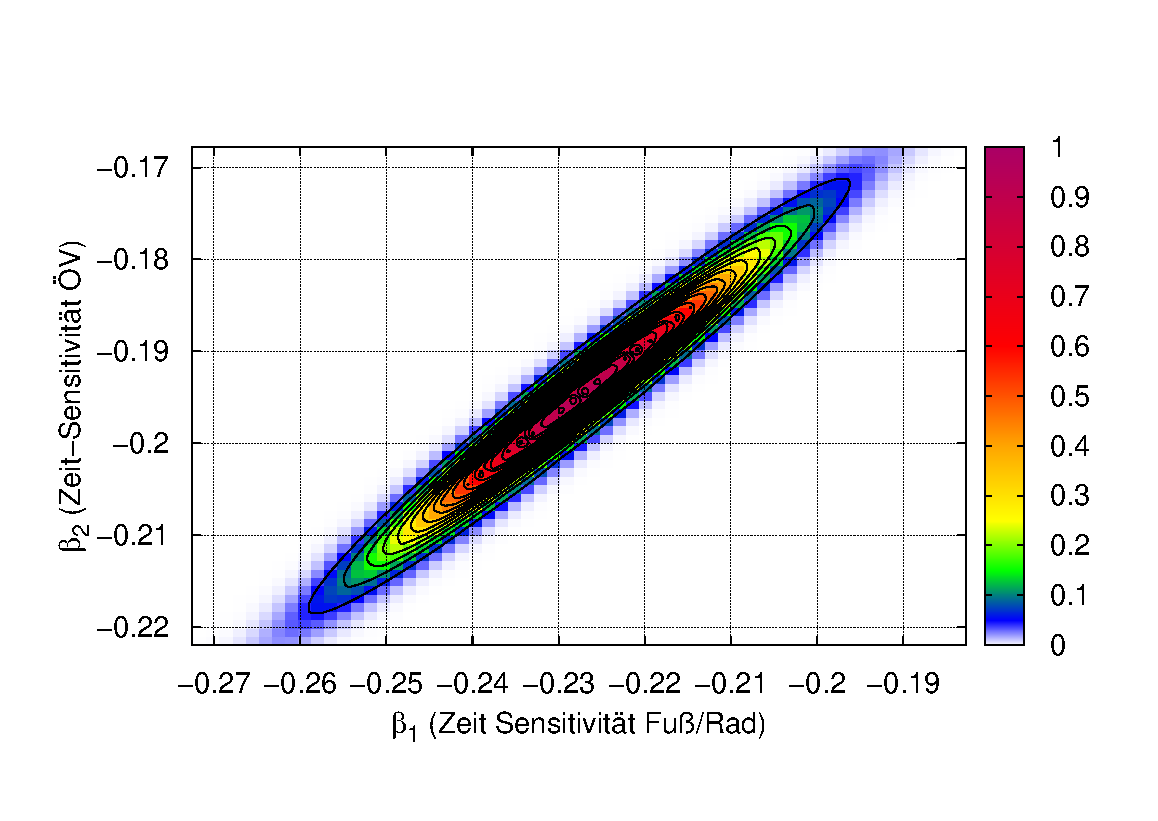
\includegraphics[width=0.50\textwidth]{figsErh/VkoekSS09_statedChoice_Lbeta1beta2.eps}
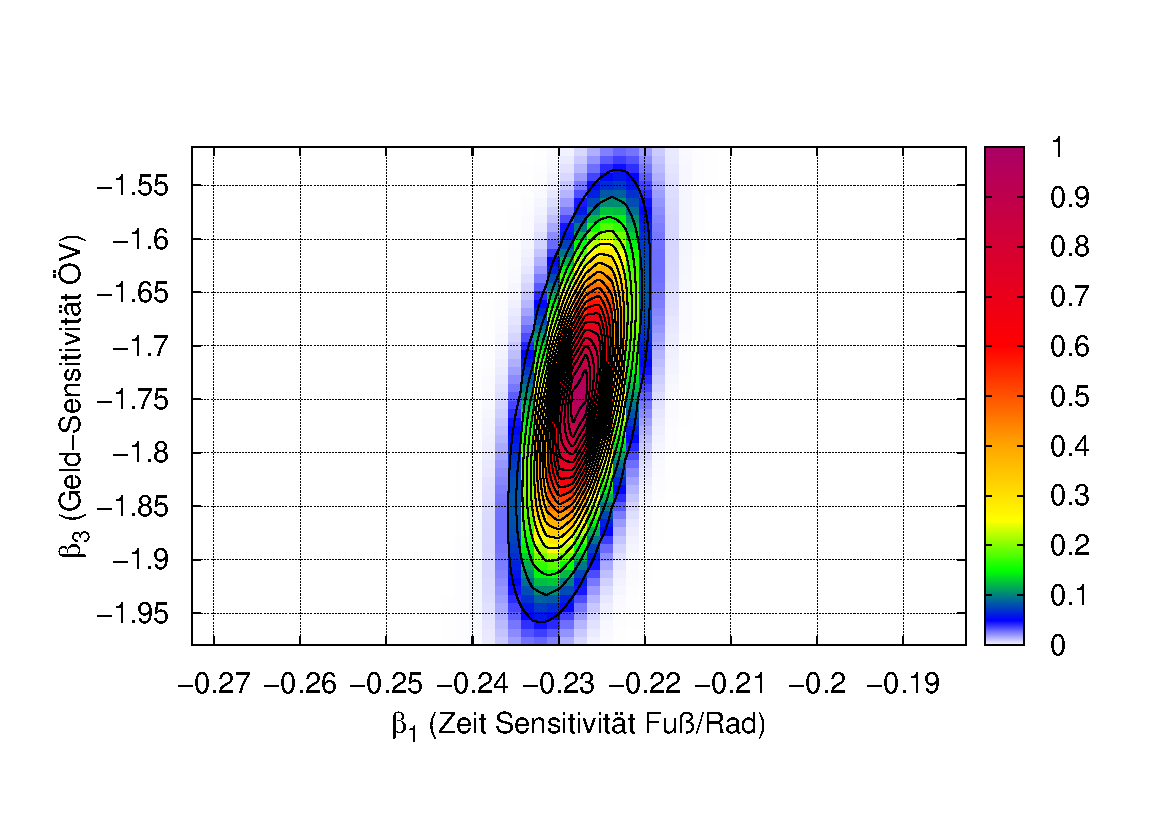
\includegraphics[width=0.50\textwidth]{figsErh/VkoekSS09_statedChoice_Lbeta1beta3.eps}
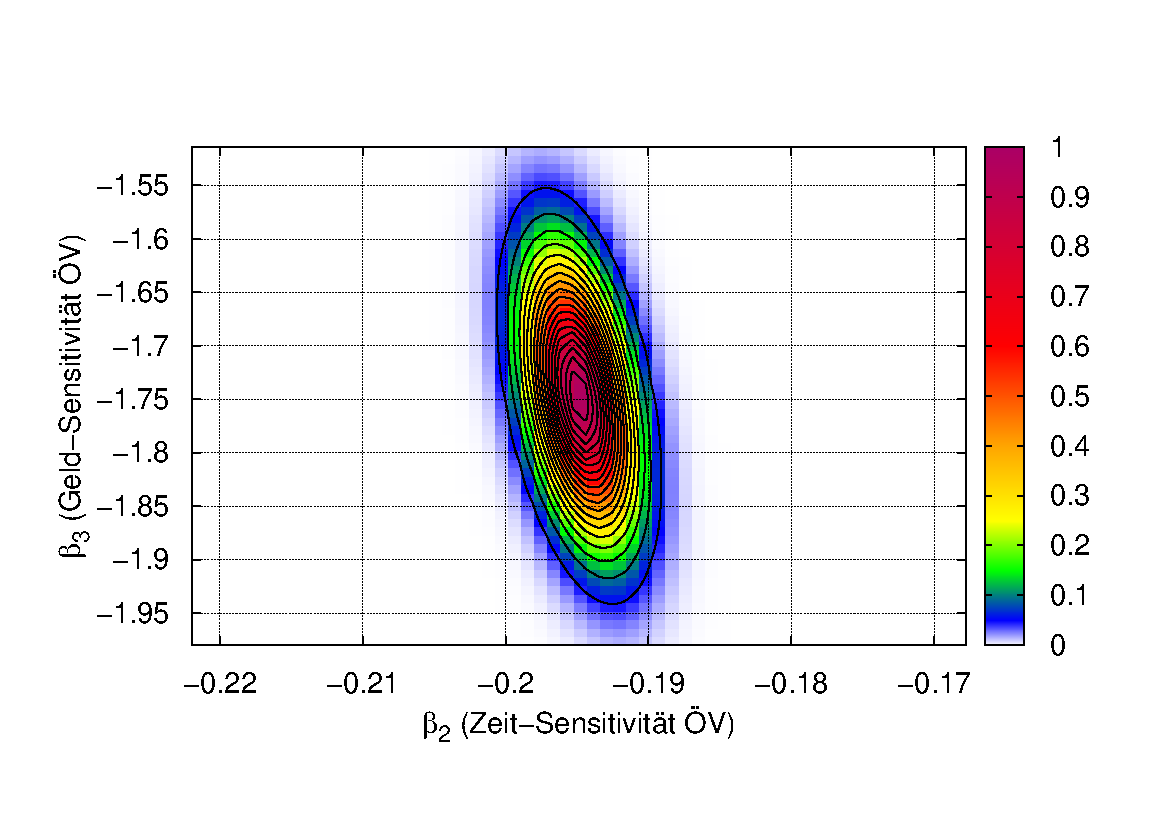
\includegraphics[width=0.50\textwidth]{figsErh/VkoekSS09_statedChoice_Lbeta2beta3.eps}
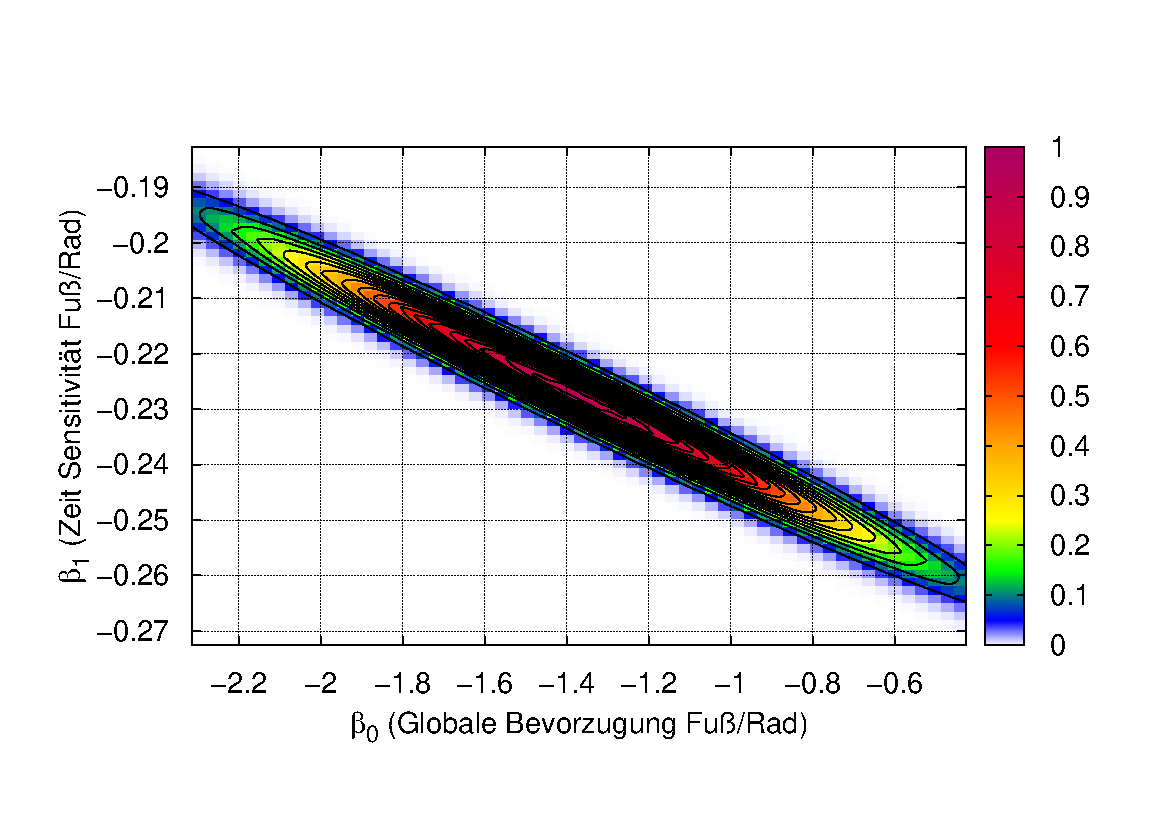
\includegraphics[width=0.50\textwidth]{figsErh/VkoekSS09_statedChoice_Lbeta0beta1.eps}
\caption{\label{fig:statedChoice_beta} Likelihoodfunktionen von
Parameterkombinationen nach der in Kap.~\ref{sec:discrKalib}
besprochenen Methode. Die Bilder zeigen die auf ein Maximum von 1
skalierte Wahrscheinlichkeitdichte daf\"ur, dass das aus den
Nutzenfunktionen~\refkl{V1V2} formulierte Logit-Modell die Daten der
Tabelle~\ref{tab:statedChoice} beschreibt. Jeweils zwei Parameter
variieren und die anderen beiden werden
jeweils auf ihren gesch\"atzten Wert gehalten.}
% werden. Jeder Plot hat einen Wertebereich,
%welcher zwei Standardabweichungen um den Sch\"atzwert
%(=wahrscheinlichsten Wert) des jeweiligen Parameters 
%liegt. Die Tatsache, dass z.B. $\beta_1$ im
%Plot rechts unten eine scheinbar viel kleinere Streuung hat, liegt in
%Wirklichkeit an der Projektion.}
\end{figure}
%###################################



\bi
\item Unsch\"arfe des Zufallsnutzens in Fu\3/Rad-Minuten:
$
-\frac{1}{\beta_{1}}=4.4
$

\item Unsch\"arfe des Zufallsnutzens in \"OPNV-Minuten:
$
-\frac{1}{\beta_{2}}=5.1
$

\item Unsch\"arfe des Zufallsnutzens in \"OPNV-\euro{}:
$
-\frac{1}{\beta_{3}}=0.57
$

\item Bonus des \"OV in Einheiten der Standardabweichung des
  Zufallsnutzens: 
$
-\beta_{0}=1.4
$

\item Bonus des \"OV  in \"OV-Minuten:
$
-\frac{\beta_{0}}{\beta_{2}}=7.0
$


\item Geldbewertung der \"OV-Kosten in \euro{}/\"OV-Stunden:
   $
\frac{60 \ \beta_{2}}{\beta_{3}}=6.7
$
\ei



Die Ergebnisse direkter Nutzenmessungen bzw. die dazugeh\"origen
Modellaussagen kann man auch als Kontourplots
darstellen: \"Uber einen Unterraum der exogenen Variablen
(z.B. Reisezeiten, Kosten) werden 
Isolinien konstanter Auswahlwahrscheinlichkeiten dargestellt, vgl.
Abb. \ref{fig:statedChoiceContour}. Hierbei sieht man die Grenzen des
auf konstanter Schwan\-kungsbreite des Zufallsnutzens beruhendem
Logit-Modell. In Realit\"at nimmt wohl die Unsch\"arfe des
Zufallsnutzens mit den Absolutwerten der Zeiten zu, wodurch die
Isolinien qualitativ so wie in Abb. \ref{fig:statedChoiceContour}
rechts aussehen, also insbesondere nicht wie beim Logitmodell parallel
zueinander sind (Abb. \ref{fig:statedChoiceContour} links). 


%###################################
\begin{figure}
\includegraphics[width=0.50\textwidth]{figsErh/VkoekSS09_statedChoice_5.eps}
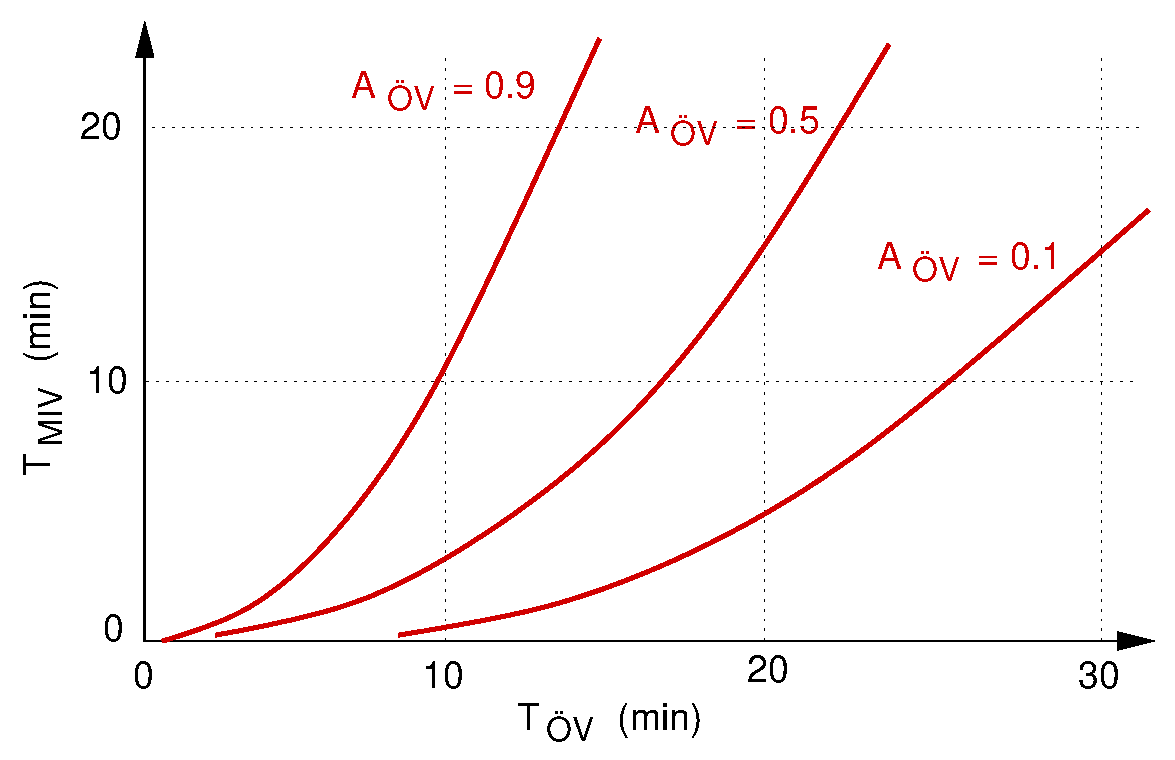
\includegraphics[width=0.50\textwidth]{figsErh/StatedChoice.eps}
\caption{\label{fig:statedChoiceContour} Kontourplot der Anteilswerte f\"ur
die Alternative ``\"OPNV'' in Abh\"angigkeit der Widerstandsfunktionen
(negative Nutzen) der zwei Alternativen. Links: Auf das
Umfrageergebnis kalibrierte Logit-Modell; Rechts: So sieht es wohl
realistischerweise eher aus.
}
\end{figure}
%###################################

\subsection{Komplexeres Beispiel aus der Literatur: Modal-Split in der Schweiz}
Als Beispiel, was mit dieser Methode alles erfragbar ist, werden hier
noch einige Ergebnisse einer Schweizerischen Untersuchung
(Intl. Verkehrswesen, 9/2003) wiedergegeben:

\begin{center}
\begin{tabular}{|c||r|r|}
\hline
Merkmal & Durchschnitt & gesch\"aftlicher Verkehr \\ \hline\hline
Zeitwert MIV & \unit[27.7]{Sfr/h} & \unit[74.6]{Sfr/h} \\ \hline
Zeitwert \"OPNV & \unit[18.5]{Sfr/h} & \unit[55.8]{Sfr/h} \\ \hline
1 $\times$ Umsteigen & \unit[7.6]{Sfr} & \\ \hline
Verl\"asslichkeit & \unit[0.1]{Sfr/\% Versp\"atungswahrsch.} & 
   \unit[0.7]{Sfr/\% Versp\"atungswahrsch.}  \\ \hline
\end{tabular}
\end{center}
%
Der Zeitwert des \"OPNV ist also, genau wie bei unserer 
``kleinen Untersuchung'', niedriger als der f\"ur IV. Die absoluten
Werte sind aber in der Schweizer Untersuchung tendenziell h\"oher, was wohl
an den sozio\"okonomischen Variablen liegt: Schlie\3lich ist die
Schweiz teuer und die befragten Personen waren nicht nur
Studenten. Diese Abh\"angigkeit wird auch durch den gro\3en
Unterschied der Bewertung von gesch\"aftlichen und sonstigen Verkehr
(Wegezweck!) deutlich. Bemerkenswert ist auch, dass einmal
Umsteigen mit 7.5 Sfr bewertet wird, zus\"atzlich zum Zeitverlust,
welcher bereits im Zeitwert enthalten ist. Schlie\3lich f\"allt auf,
dass beruflich T\"atige die Zuverl\"assigkeit drastisch h\"oher
gewichten als der Durchschnitt.


\aufgabenbox{Aufgabe:}{Wie w\"achst in dem durch \refkl{V1V2} und
\refkl{StatedChoiceLogit} definierten Entscheidungsmodell die
Entscheidungsunsch\"arfe mit den Absolutwerten der Zeitaufw\"ande an?
Ist insbesondere die absolute Unsch\"arfe $\Delta V$ oder die relative
Unsch\"arfe $\Delta V/V$ konstant? Ist das Ergebnis aus
Abb. \ref{fig:statedChoice} und
\ref{fig:statedChoiceContour}  konsistent mit diesem Modell?
}


%####################################
\subsection{Experimentelles Design der Choice Sets}
%####################################

Prinzipiell besteht eine wahlbasierte Conjoint-Untersuchung aus vier
Schritten
\benum
\item Modellspezifikation, insbesondere welche Alternativen und welche
  exogenen Variablen ber\"ucksich\-tigt werden,
\item Experimentelles Design: Wieviele Choice Sets sollen es sein? Welchen
  Wertebereich haben die exogenen 
  Variablen? Bekommt jeder Proband dieselbe Menge an Choice Sets?
  Welche  Wertekombinationen werden den Choice Sets
  zugeordnet?
\item Erstellung der Fragek\"artchen (jedes Choice Set auf ein
  eigenen K\"artchen, bei Pivotstudien ggf. individualisiert f\"ur die
  einzelnen Befragten) und Durchf\"uhrung der Befragung
\item Auswertung
\eenum
%
Das experimentelles Design zielt daraufhin, die Choice Sets so
auszuw\"ahlen, dass die Analyse des diskreten Wahlmodells 
 bei m\"oglichst geringer Anzahl der Sets (mehr als
15 bis 20 kann man Probanden kaum zumuten) unverzerrte und
m\"oglichst scharfe Aussagen erlaubt. Dabei werden, um die
Probanden nicht zu verwirren, auch
kardinalskalierte Variablen meist nur in wenigen Auspr\"agungen
vorgegeben. F\"ur die Studentenbefragung des
Abschnitts~\ref{sec:erh-studiBsp} (Wahl zwischen den zwei Alternativen
Fu\3/Rad und \"OV) k\"onnte man beispielsweise folgende Stufen definieren:
\bi
\item Komplexe Reisezeit $T_1$ der Alternative Fu\3/Rad: 10, 15, 20, 25 und 30
  Minuten,
\item Komplexe \"OV-Reisezeit  $T_2$: 10, 15, 20, 25 und 30
  Minuten,
\item Ad-Hoc-Kosten $K_2$ des \"OV: 0.00, 1.50, 3.00 oder 4.50 Euro
\ei
Bei Pivot-Designs (Ausgangspunkt sind Revealed Choice Befragungen)
k\"onnte man auch feste Prozentstufen bez\"uglich der tats\"achlichen
Auspr\"agungen (z.B. Preis wie bisher, \unit[20]{\%} billiger oder
teurer,  \unit[40]{\%} teurer) w\"ahlen. 
Es gibt drei wesentliche Strategien zur Auswahl der Choice Sets:
\vspace{1em}

\noindent
\bfdef{Vollst\"andige Enumeration 
(\emph{full factorial  design})}:
 Es werden alle m\"oglichen Kombinationen angewandt:
\begin{center}
\begin{tabular}{|r|c|c|c|} \hline
$i$ & Fu\3-Rad Reisezeit $T_1$ & \"OV-Reisezeit  $T_2$ & \"OV Ad-Hoc-Kosten $K_2$
   \\ \hline
1 & \unit[10]{min} & \unit[10]{min} & \unit[0.00]{\euro{}}\\
2 & \unit[10]{min} & \unit[10]{min} &\unit[1.50]{\euro{}}\\
\vdots & \vdots & \vdots & \vdots  \\
99 & \unit[30]{min} & \unit[30]{min} & \unit[3.00]{\euro{}}\\
100 & \unit[30]{min} & \unit[30]{min} & \unit[4.50]{\euro{}}\\
 \hline
\end{tabular}
\end{center}
Hier sind es also $n=5\times 5 \times 4=100$ Choice Sets.
\vspace{1ex}

\noindent
\textit{Vorteile}:
\bi
\item Maximale Trennsch\"arfe, alle Arten von Kreuz-Effekten werden so
  gut wie m\"oglich ber\"ucksich\-tigt
\ei
\textit{Nachteile}:
\bi
\item Meist prohibitiv viele Choice Sets
\item Viele \"uberfl\"ussige Fragen (triviale Sets), bei denen die
  Wahl offensichtlich ist wie im Set~20, bei dem man die Auswahl hat
  zwischen   einen Fu\3weg von 
  \unit[10]{Minuten} oder den \"OV, wenn dieser
  \unit[30]{Minuten} dauert sowie zus\"atzlich \unit[4.50]{\euro{}} kostet.
\ei

\vspace{1em}

\noindent
\bfdef{Orthogonales Design}: Die Merkmalskombinationen werden so
gew\"ahlt, dass es keine deskriptiven Korrelationen gibt. Schreibt man
die Tabelle der Choice Sets abstrakt als normalisierte Datenmatrix $\m{X}$ (die
Zeilen sind die einzelnen Choice Sets und die Spalten sind $T_1-\overline{T}_1$,
$T_2-\overline{T}_2$ und $K-\overline{K}$ (bzw. die  auf das
arithmetische Mittel 0 normalisierten 
Stufenindices von $T_1$, $T_2$ und $K$), so
enth\"alt die Kovarianzmatrix
 $(\m{X}\tr\m{X}/n$ keine
Nichtdiagonalelemente. Beispiel: Das Design
\begin{center}
\begin{tabular}{|r|c|c|c|} \hline
$i$ & Fu\3-Rad Reisezeit $T_1$ & \"OV-Reisezeit  $T_2$ & \"OV Ad-Hoc-Kosten $K_2$
   \\ \hline
2 & \unit[10]{min} & \unit[10]{min} & \unit[1.50]{\euro{}}\\
18 & \unit[10]{min} & \unit[30]{min} & \unit[1.50]{\euro{}}\\
84 & \unit[30]{min} & \unit[10]{min} &\unit[3.00]{\euro{}}\\
99 & \unit[30]{min} & \unit[30]{min} &\unit[3.00]{\euro{}}\\
\hline
\end{tabular}
\end{center}
ist orthogonal bez\"uglich der Attributstufen innerhalb einer
Alternative, aber nicht zwischen den Alternativen (die Fu\3/Rad Zeit
$T_1$ ist positiv mit den \"OV-Kosten $K_2$ korreliert). 
\vspace{1ex}

\noindent
\textit{Vorteile}:
\bi
\item Orthogonal
\ei
\textit{Nachteile}:
\bi
\item Meist immer noch zu viele Choice Sets, wenn man hinreichende
  Genauigkeit will
\item Weiterhin viele triviale Sets, zumindest, wenn man auch zwischen
  den Alternativen Orthogonalit\"at vorschreibt (dann ben\"otigt man
  im obigen Beispiel mindestens acht Choice Sets, u.A. Set~19, bei dem man die Auswahl hat
  zwischen 
  einen Fu\3weg von 
  \unit[10]{Minuten} oder \"OV, wenn dieser
  \unit[30]{Minuten} dauert sowie zus\"atzlich \unit[3.00]{\euro{}} kostet.
\item Orthogonalit\"at, zumindest zwischen Alternativen, ist
  eigentlich sinnlos, da die \emph{ Differenzen}
  zwischen den Attributen entscheidend ist.
\ei



\vspace{1em}

\noindent
\bfdef{Effizientes Design}: Dies ist die einzige Strategie, bei der
man die Zahl $n$ der Choice Sets explizit vorgeben kann. Unter allen
 Designs (also Mengen mit $n$ Sets, deren Anzahl ist in obigem Beispiel bei
$n=10$ immerhin $\ueber{10}{100} > 10^{12}$)
 ist das effiziente Design dasjenige, welches bei der Auswertung mit
 dem diskreten Wahlmodell die geringsten Unsicherheiten bei den
 Parametersch\"atzern ergibt. Daf\"ur wird \"ublicherweise das Ma\3 des
 \bfdef{D-errors} (\emph{determinantenbasierte Ungenauigkeit})
\be
\label{D-error}
D\sub{err}=\text{det}\left[\left(\m{V}_{\hatvecbeta}\right)^{1/J}\right]
\ee
herangezogen, also das geometrische Mittel der Hauptkomponenten der
Varianz-Ko\-va\-ri\-anz-Matrix der  $J$ Parametersch\"atzer. Die Sch\"atzer,
$\hatvecbeta$, ebenso wie die Varianz-Kovarianz-Matrix
$\m{V}_{\hatvecbeta}$,  werden  mit dem
\emph{Maximum-Likelihood-Verfahren} gewonnen (welches erst 
 in Abschnitt~\ref{sec:discrStat} n\"aher betrachtet wird). Das
 impliziert aber auch, dass man zumindest eine ungef\"ahre Vorstellung
 der eigentlich erst durch die Befragung zu ermittelnden Parameter
 haben muss. 

\vspace{1ex}

\noindent
\textit{Vorteile}:
\bi
\item Frei w\"ahlbare Anzahl der Choice Sets
\item maximale Trennsch\"arfe
\ei
\textit{Nachteile}:
\bi
\item Um den \emph{D-error} zu berechnen, ben\"otigt man eine
  vorl\"aufige Parametersch\"atzung, welche man aus der Literatur
  (oder dem \emph{Pre-Test} der Studie) entnehmen muss.
\item Die Ermittlung des effizienten Designs is numerisch aufw\"andig.
\ei

